\emph{Groupe témoin de \np{1000} bovins : 200 malades (180 testés positifs, 20 négatifs) et
800 non malades (45 positifs, 755 négatifs) ; au total 225 tests positifs.
On note $M$ l'évènement \og le bovin est malade \fg{} et $T$ l'évènement \og le test est positif \fg.}

\begin{enumerate}
	\item Le bovin est choisi au hasard : on est en situation d'équiprobabilité.
	\[P(M) = \dfrac{200}{\np{1000}} = 0,2.\]

	\item $M \cap T$ : \og le bovin est malade et son test est positif \fg.
	\[P(M \cap T) = \dfrac{180}{\np{1000}} = 0,18.\]
	La probabilité que le bovin soit malade et que son test soit positif est égale à $0,18$.

	\item Parmi les 200 bovins malades, 180 ont un test positif :
	\[P_M(T) = \dfrac{180}{200} = 0,9.\]

	\item \og Ne pas être atteint sachant que le test est positif \fg{} se traduit par
	$P_T\left(\overline{M}\right)$. Parmi les 225 bovins testés positifs, 45 ne sont pas malades :
	\[P_T\left(\overline{M}\right) = \dfrac{45}{225} = \dfrac{45}{5 \times 45} = \dfrac{1}{5} = 0,2.\]
	Or $0,2 > 0,15$ : le test \textbf{n'est pas fiable}.

	\item
	\begin{enumerate}
		\item Le tirage est assimilé à un tirage avec remise : à chaque niveau,
		$P(M) = 0,2$ et $P\left(\overline{M}\right) = 1 - 0,2 = 0,8$.

		\begin{center}
			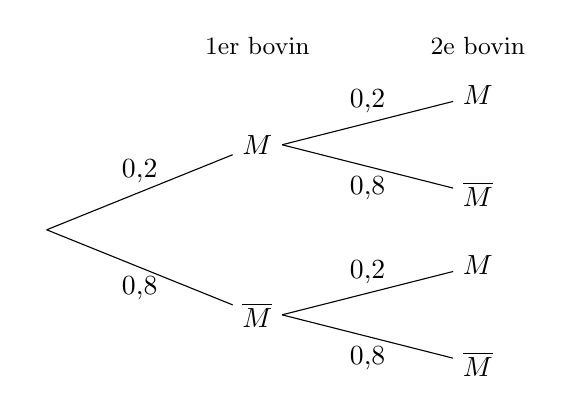
\begin{tikzpicture}[x=2.8cm, y=0.9cm]
				
				\node (root) at (0,0) {};
				\node (M) at (1,1.2) {$M$};
				\node (Mb) at (1,-1.2) {$\overline{M}$};
				\node (M1) at (2,1.9) {$M$};
				\node (M1b) at (2,0.5) {$\overline{M}$};
				\node (M2) at (2,-0.5) {$M$};
				\node (M2b) at (2,-1.9) {$\overline{M}$};
				
				\draw (root.east) -- (M) node[pos=0.5,above] {0,2};
				\draw (root.east) -- (Mb) node[pos=0.5,below] {0,8};
				
				\draw (M.east) -- (M1) node[pos=0.5,above] {0,2};
				\draw (M.east) -- (M1b) node[pos=0.5,below] {0,8};
				\draw (Mb.east) -- (M2) node[pos=0.5,above] {0,2};
				\draw (Mb.east) -- (M2b) node[pos=0.5,below] {0,8};
				
				\node at (1,2.6) {\small 1\up{er} bovin};
				\node at (2,2.6) {\small 2\up{e} bovin};
			\end{tikzpicture}
		\end{center}

		\item L'évènement $A$ correspond au chemin $M$ -- $M$ de l'arbre :
		\[P(A) = 0,2 \times 0,2 = 0,04.\]
		La probabilité que les deux bovins choisis soient malades est égale à $0,04$.
	\end{enumerate}
\end{enumerate}
